\chapter{Visual recognition}
The pictures are valuable to accurately determine the emotion of the user. For instance, happy photos might contain sunny landscapes and sandy beaches while sad pictures might contain darker colors. To analyse the images, we'll use convolutional neural networks, which achieve state-of-the-art performances in many visual recognition tasks. First we'll explain how they work and then we'll dive into the architecture we've used for deep sentiment analysis.
%%%%%%%%%%%%%%%%%%%%%%%%%%%%%%%%%%%%%%%%%%%%%%%%%%%%%%%%%%%%
%%%%%%%%%%%%%%%%%%%%  NEW SECTION   %%%%%%%%%%%%%%%%%%%%%%%%
%%%%%%%%%%%%%%%%%%%%%%%%%%%%%%%%%%%%%%%%%%%%%%%%%%%%%%%%%%%%
\section{Convolutional neural networks}
A convolutional neural network, often called ConvNet, can be seen as a simulation of the human visual cortex, that is to say an aggregation of plenty of receptive fields. (some illustrations might be helpful here)

\subsection{Convolutional layer}
Take an image of dimension $(h,w,3)$ with $h$ the height, $w$ the width and 3 representing the number of channels (red, blue, green). If you simply flatten that image and transform it into a vector of size $h\times h \times 3$ and feed that vector to a neural network, you'll get average results as you've thrown away all the spatial information. Convolutions extract that spatial information and work the following way:
\begin{itemize}
    \item Each convolution is described by a filter F of size $(f, f, 3)$, $f$ usually being equal to 3, 5, or 7.
    \item Position the filter on the upper left of the image and element-wise multiply with the filter, then sum those numbers to obtain a `neuron'.
    \item Slide across the image, one pixel at a time horizontally and vertically, and repeat the previous operation (see Figure \ref{convolution}).
\end{itemize}

\begin{figure}
\begin{subfigure}[t]{.5\textwidth}
  \vskip 0pt
  \centering
  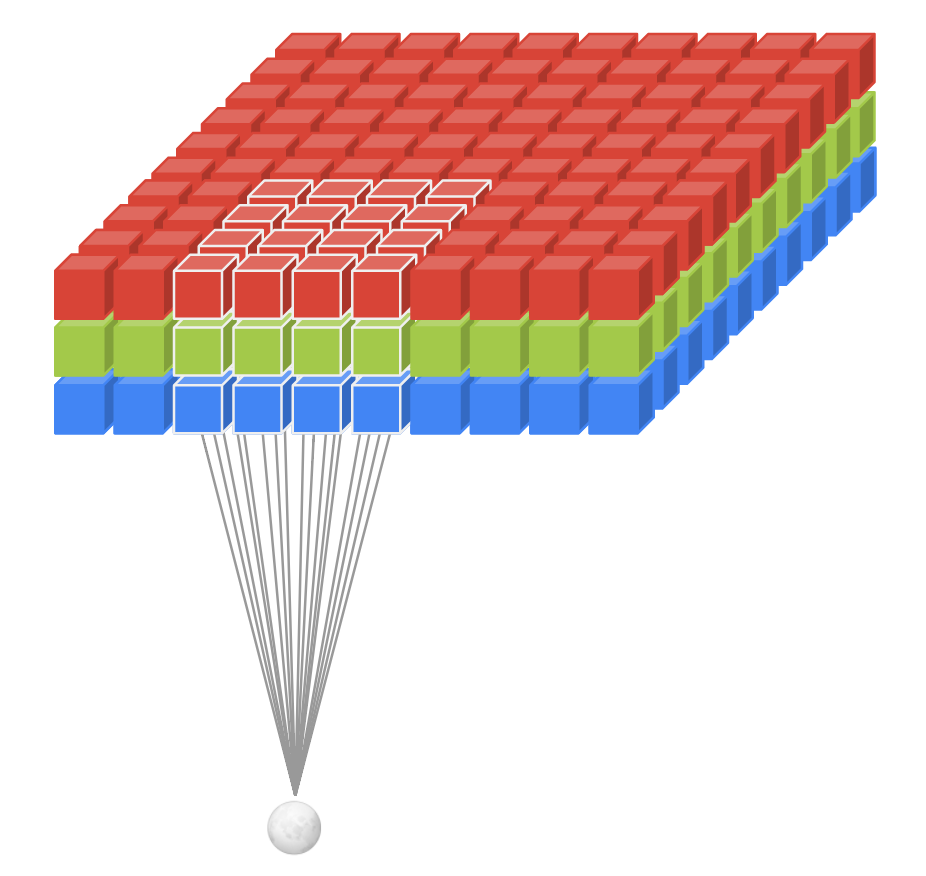
\includegraphics[width=.8\linewidth]{Images/conv1.png}
  \caption{One operation of convolution}
\end{subfigure}
\begin{subfigure}[t]{.5\textwidth}
  \vskip 0pt 
  \centering
  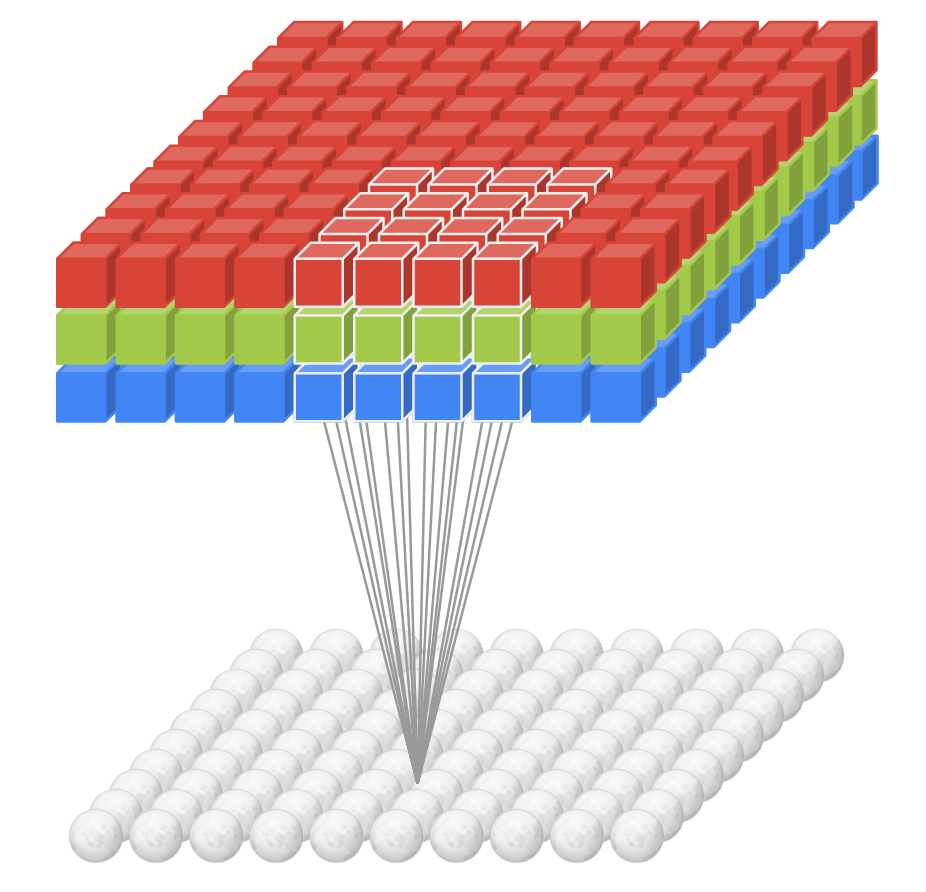
\includegraphics[width=.8\linewidth]{Images/conv2.png}
  \caption{The result of the convolution}
\end{subfigure}
\caption{A convolution, each neuron been a `receptive field' \cite{gorner}}
\label{convolution}
\end{figure}

By sliding through the image, you will get a new matrix of dimension $(h_{new}, w_{new},1)$, with $h_{new}=h-f+1$ and $w_{new}=w-f+1$. However, we usually don't want to reduce the size of our input image that fast, as we want to stack several convolutions. To ensure that the image has the same size after each convolution, zero-padding is used: we add $p$ zeros to the borders of the input image to preserve the spatial size of the input. (illustration needed, before and after zero-padding)With zero-padding, $h_{new}$ becomes: $h_{new} =  h + 2p - f + 1$, and we want that $h_{new}$ to be equal to $h$:
\begin{equation}
h + 2p - f + 1 = h
\end{equation}
Therefore, $p=\frac{f-1}{2}$. Besides, zeros are used instead of any other number because you want the filter to activate on the pixels of the image only, therefore, setting the added border to zeros ensure that the resulting neuron will not be influenced by the border.

A convolution extracts information about the image such as edges or blotches of some color (Figure \ref{conv-ex}). The grayscale and edges filters were hardcoded but in a ConvNet setting, the weights of the filter F are learned through optimising a loss function -- in our case, a metric measuring how accurate our predictions of the emotions are. The network will learn weights that will detect features that will be most relevant to our specific task. A convolution also has a depth parameter $d$: simply repeat the operation described above $d$ times with $d$ independent filters of the same size $(f, f, 3)$, to create a new tensor of dimension $(h,w,d)$.

We can then apply convolutions on that new tensor. First layers will detect simple features such as edges or aggregation of colors, and deeper layers might recognise more complex features such as faces or wheels.

\begin{figure}
\centering
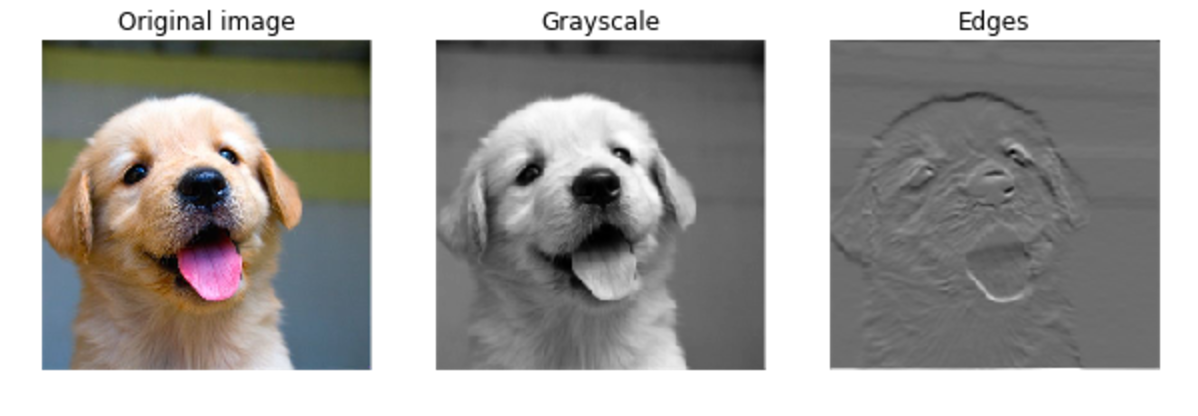
\includegraphics[width=0.8\textwidth]{Images/conv_ex.png}
\caption{Examples of convolution}
\label{conv-ex}
\end{figure}

\subsection{ReLU layer}
Stacking convolutions is nice, but as it is, we are only creature features that are linearly dependent of the input pixels: we could in fact replace all the convolutions with a single matrix multiplication. In order to learn more interesting functions, we have to add non-linearities. Historically, the popular choice was the sigmoid function defined as:
\begin{equation}
\text{sigmoid}(x) = \frac{1}{1+e^{-x}}
\end{equation}

\begin{figure}[H]
\centering
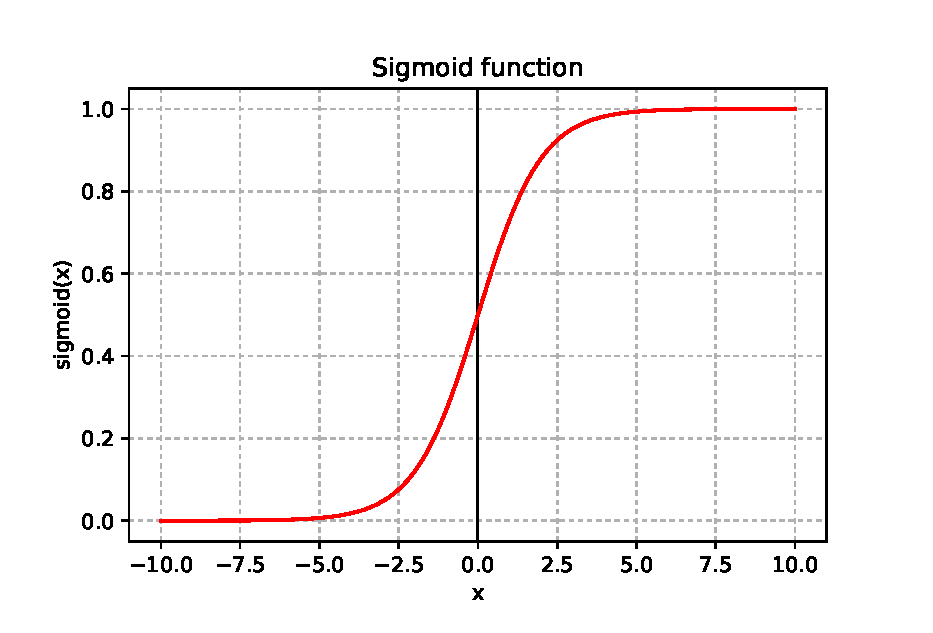
\includegraphics[width=0.5\textwidth]{Images/sigmoid.eps}
\caption{Sigmoid function}
\end{figure}

The sigmoid function is the simplest function having values between 0 and 1 mimicking the biological neurons `firing' in reaction to their inputs. However, when the network is learning to minimise a loss function through backpropagation, the gradients tend to vanish to zero as the sigmoid's derivative goes to zero for high negative and positive values. The most popular choice of non-linearity is now the Rectified Linear Unit (ReLU) defined as:
\begin{equation}
\text{ReLU}(x) = \text{max}(0,x)
\end{equation}

\begin{figure}[H]
\centering
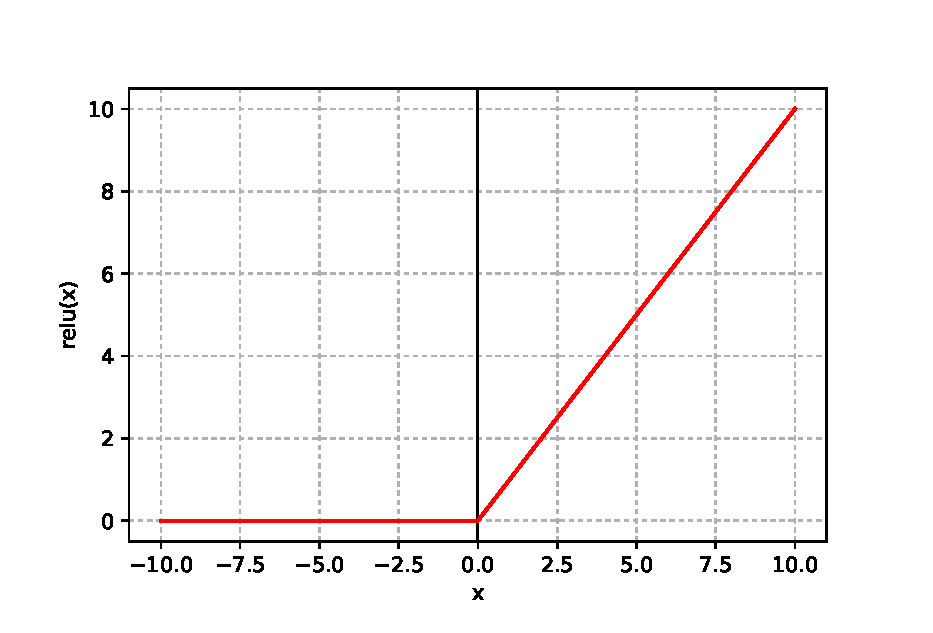
\includegraphics[width=0.5\textwidth]{Images/relu.eps}
\caption{ReLU function}
\end{figure}

The ReLU's gradient is non-saturating for highly excited neurons which turns out to be a nice property to learn faster. In the network, each layer of convolution is followed by a ReLU layer, that simply applies the function $\text{max}(0,x)$ to each neuron.

\newpage
\subsection{Pooling layer}
There is a lot of spatial redundancy in an image, we don't need all the pixels to be able to identify what's in a picture. For example we can perfectly identify the animal in Figure \ref{kittens} by reducing the number of pixels by two.

\begin{figure}[H]
\centering
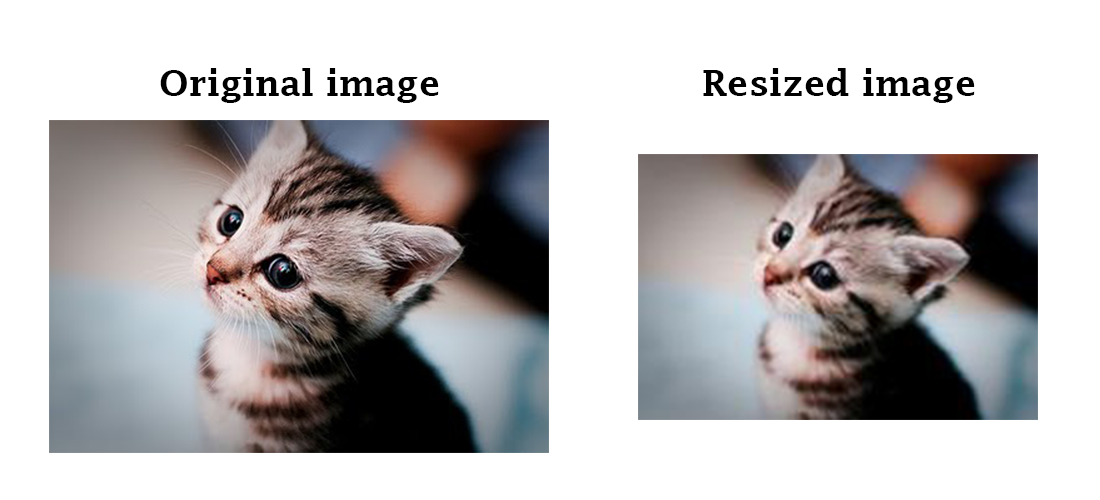
\includegraphics[width=0.8\textwidth]{Images/kittens.png}
\caption{A kitten, and the same kitten with half the pixels}
\label{kittens}
\end{figure}

The same idea applies to convolved images, we might not need all the neurons that were created. The pooling operation downsamples the image in the following way:
\begin{itemize}
    \item Pick a channel among the $d$ ones.
    \item Position yourself on the top-left 2x2 square of the image and take the max.
    \item Repeat by sliding through the image vertically and horizontally with a stride/step of 2 (see Figure \ref{maxpool}).
\end{itemize}

\begin{figure}[H]
\centering
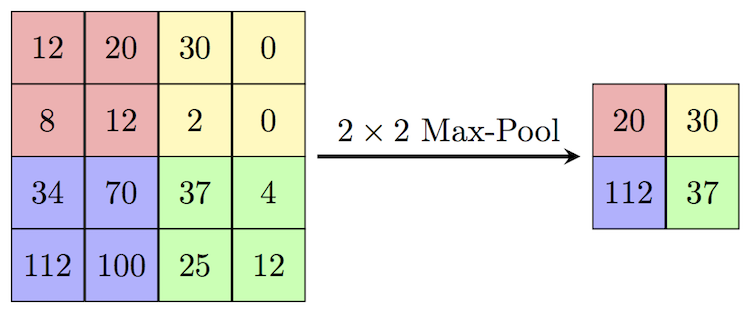
\includegraphics[width=0.8\textwidth]{Images/maxpool.png}
\caption{Max pooling \cite{camb-spark}}
\label{maxpool}
\end{figure}

After applying max pooling to each channel, the resulting image dimension is $(\frac{h}{2}, \frac{w}{2}, d)$ and we have discarded 75\% of the neurons (as in each max-pool operation, we only keep the maximum neuron among the fours), effectively reducing the number of parameters and controlling overfitting.

You could wonder why max-pooling and not average pooling (taking the mean value of the four neurons)? The convolutions allow us to see if a certain feature is in the image when a neuron fires, and we only want to know if that feature is there in a certain region. Therefore taking the max of the four neurons is sufficient to know whether that feature is there or not in that particular region.

In practice, after a few iterations of convolutions, inserting pooling layers in-between convolutional layers might be a good idea to control the spatial complexity of the network.

\subsection{An example of convolutional network}
Here is an example of a convolutional neural network with an input image of size $(224, 224, 3)$:

\begin{figure}[H]
\centering
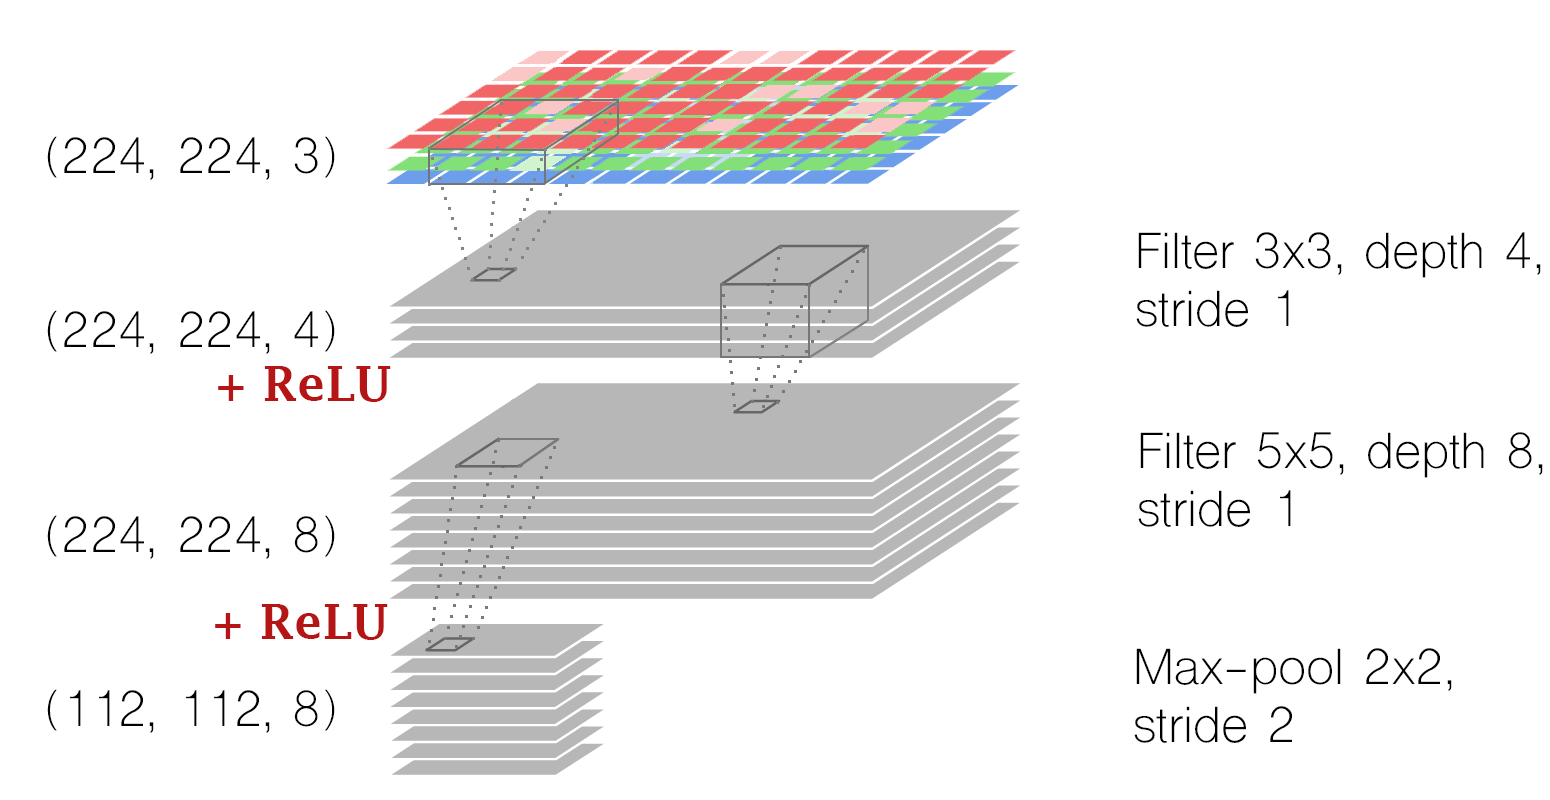
\includegraphics[width=0.8\textwidth]{Images/conv_archi.png}
\caption{An architecture of a neural network \cite{gorner}}
\end{figure}

\begin{itemize}
    \item A first convolution with a filter of size $3\times3$ is applied, with depth 4, stride 1 and zero-padding of 1.
    \item A ReLU layer.
    \item A second convolution with a filter of size $5\times5$ is applied, with depth 8, stride 1 and zero-padding of 2.
    \item A ReLU layer.
    \item Max-pooling of size $2\times2$ with stride 2, reducing the height and width by 2.
\end{itemize}

After the last operation, the neurons are reshaped into a vector that can be fed to the traditional fully connected layers of neural networks.

\subsection{Deep convolutional networks}
Best results are achieved using deep convolutional networks, that is to say by stacking many layers of convolutions/ReLU/max-pool. But what exactly is `many'? Let us have a look at the main Computer Vision competition: ImageNet Large Scale Visual Recognition (ILSVR).
\begin{enumerate}
    \item \textbf{AlexNet} \cite{alexnet}: The first popular convolutional network, developed by Alex Krizhevsky, Ilya Sutskever and Geoffrey Hinton, that outperformed 
    the other competitors at ILSVR 2012 by a large margin: top-5 error of 16\% compared to the runner-up with 26\%. AlexNet has 5 convolutional layers (followed by 
    ReLU), 3 max-pool layers and 3 fully-connected layers, producing a 8-layer deep network (not counting the max-pooling as it doesn't have any parameters).
    \item \textbf{GoogLeNet} (also known as Inception)\cite{googlenet}: This is the winner of ILSVR 2014 with a top-5 error of 6.7\% . This 22-layer architecture used 
    the `Inception Module' which allowed to drastically reduce the number of parameters: from 60M for AlexNet to 4M for GoogLeNet.
    \item \textbf{ResNet} \cite{resnet}: The winner of ILSVR 2015 with a top-5 error of 3.6\% thanks to an astonishing 152 layers convolutional network. This 
    architecture features `skip connections' allowing this ultra-deep network achieve such results.

(explain Inception module, talk about computational considerations (Stanford CS231n))
\end{enumerate}

\subsection{Transfer Learning}
Training a convolutional network from scratch can be difficult as a large amount of data is needed and plenty of different architectures and hyperparameters need to be tried before finding a decent model. To circumvent that issue, you can take advantage of the pre-trained models available that learned to recognize images through near 1.2M training examples and a deep architecture that took weeks to train on multiple GPUs.

More specifically, the pre-trained networks learned to recognise features on a picture that allow it to classify the latter among the 1000 classes there are on the ImageNet dataset. Those features are combined in the final fully connected layer to make a decision. Suppose that instead of classifying an image into 1000 classes we want to label it according to 6 different emotions (happy, sad, angry, scared, surprised, disgusted). The same features can be combined in a different way to let the network take a decision on the emotion label of the image.

The process described above is called {\em Transfer Learning}: you chop off the last layer of the network and add your own layer given how many classes you have. You then freeze the weights of the other layers and only backpropagate through the newly created layer when training the network on your examples. If you have enough data, you can unfreeze more higher-level layers and backpropagate through them. One way to see why this works is that earlier features of ConvNets contain more generic features (such as edges or color blobs), while later features become more specific to the details of the classes present in the dataset. For example in ImageNet, there are many dog breeds and the later representational power might be used to distinguish those \cite{transfer}.

We will be using Google's Inception network and fine-tune the last fully-connected layer.

\subsection{Google Inception network}
After AlexNet proved that convolutional networks outperformed traditional machine learning models, the trend to achieve even better results was to build wider (more units per layer) and deeper (more layers) networks and to add dropout to address overfitting. However, bigger networks are more expensive to train (more parameters) and could not be usable for real-time prediction if a forward-pass takes more than a second for instance. Moreover, if the increased capacity is not used efficiently, for example if most added weights are close to zero, then the network added depth will be completely wasted.

To address this problem, we could replace the fully connected layers by sparse ones, even inside convolutions \cite{googlenet}. Not only would it mimic more closely biological systems, but it would also have more theoretical ground thanks to the work of Arora et al. \cite{arora}. They proved that if the probability distribution of a dataset can be represented by a large, very sparse neural network, then it's possible to build the optimal network layer after layer by clustering highly correlated neurons of the preceding layer.

Current networks architectures are not using sparse layers as the libraries are heavily optimised for dense matrix multiplication. Training sparse layers would incur considerable overhead that are not handled by today's computing infrastructures. However, the Inception module is an elegant solution to add more expressiveness to your network while keeping the number of parameters low. 

\textbf{Inception module:}
At each layer, you'd normally be facing the dilemma of choosing between $1\times 1$, $3\times 3$, $5\times5$ convolution or max-pooling:

\begin{figure}[H]
    \centering
    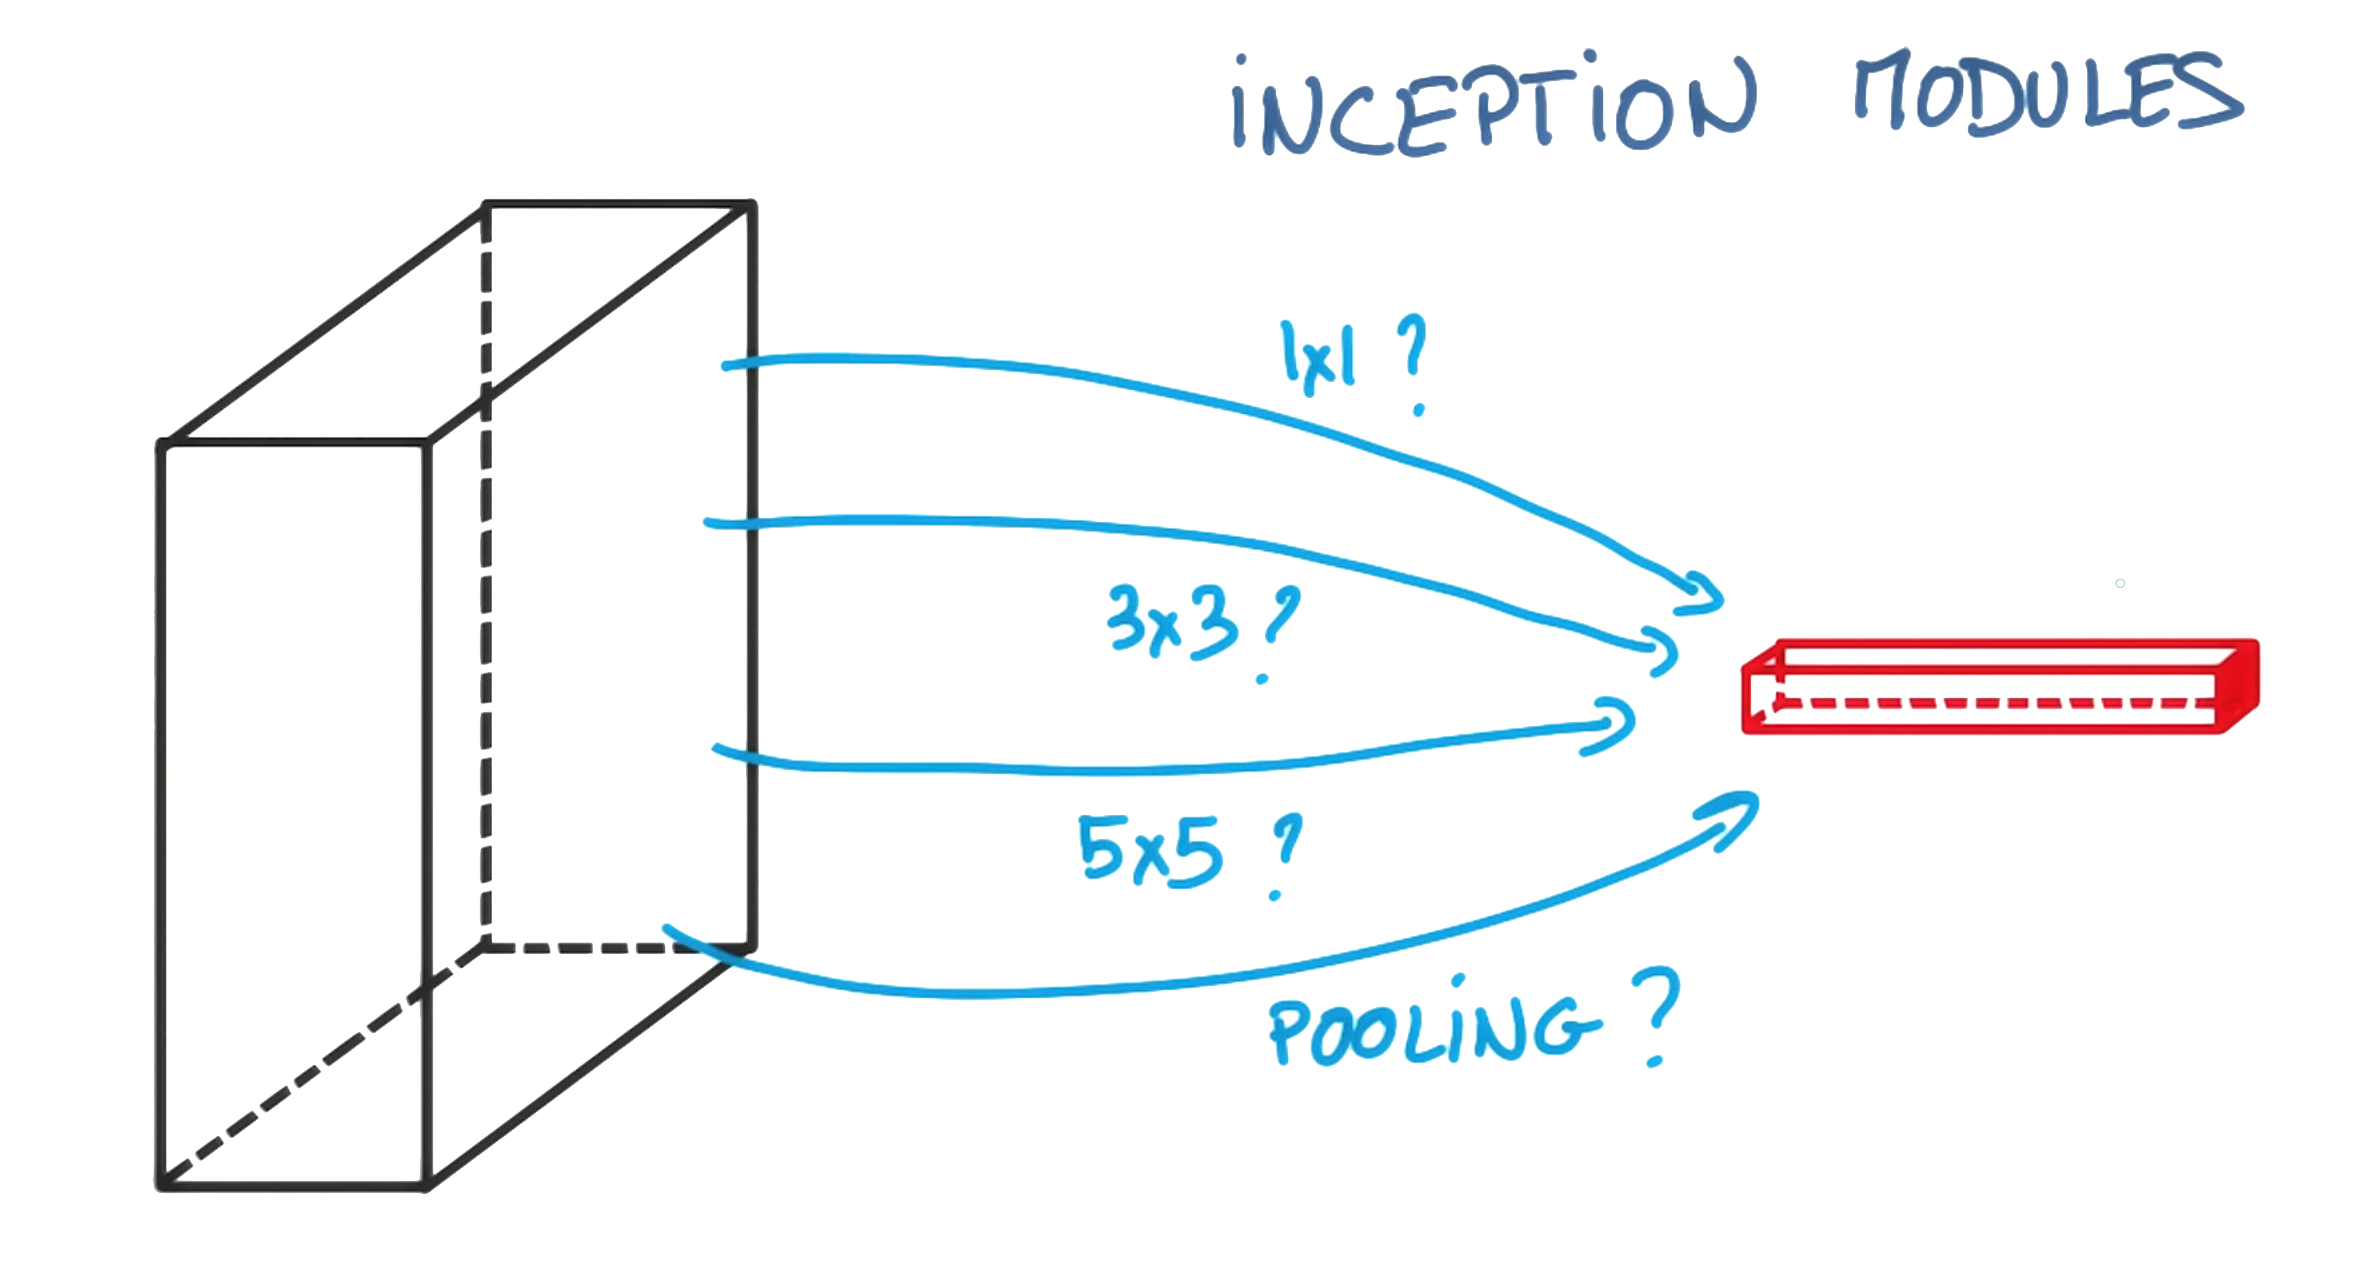
\includegraphics[width=0.8\textwidth]{Images/inceptionmodule.png}
    \caption{Which layer to choose? \cite{inceptionmodule}}
\end{figure}

In the Inception module, you perform all of the above operations and let the network decide for you. Each operation is done in parallel before being concatenated and fed to the next layer. This allows to capture both local features via small convolutions and more high-level features via large convolutions. 

\begin{figure}[H]
    \centering
    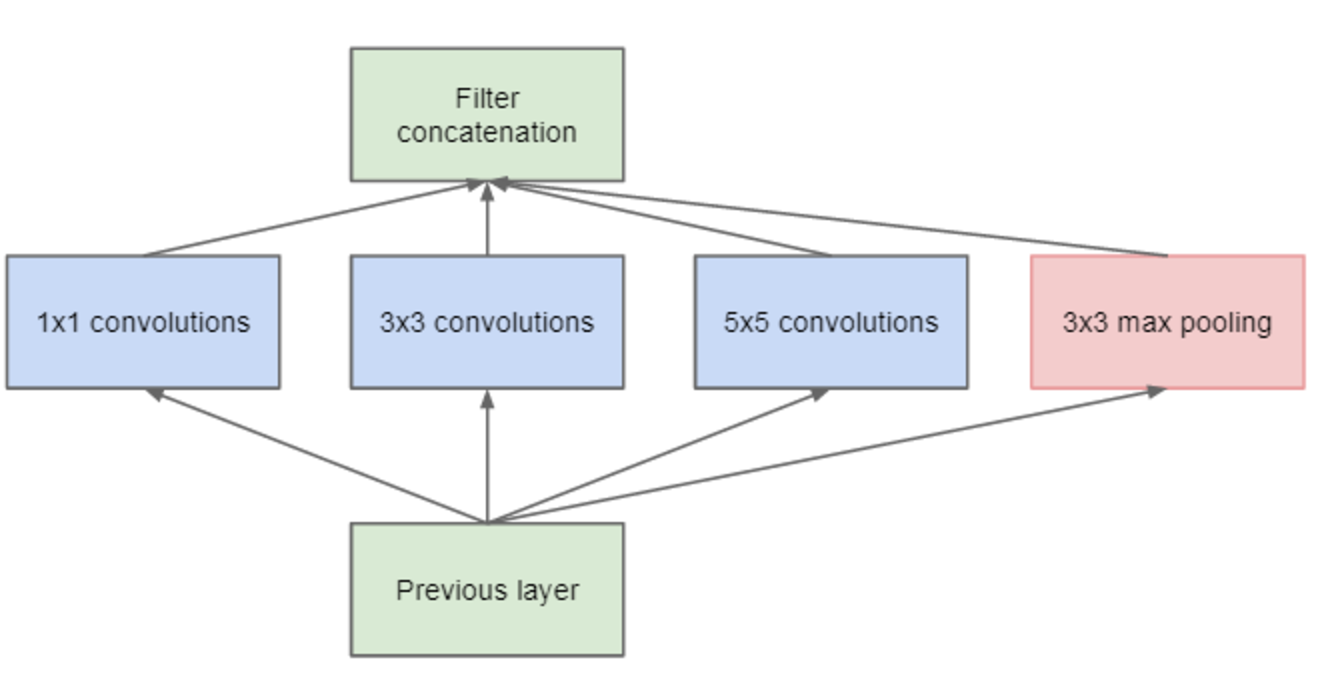
\includegraphics[width=0.8\textwidth]{Images/naiveinception.png}
    \caption{Naive Inception module \cite{googlenet}}
\end{figure}

But wait.. How is this supposed to keep the number of parameters low? This is actually the naive implementation of the Inception module. One key component are the $1\times 1$ convolution for dimensionality reduction before the large convolutions. Let's take an example to understand: suppose at an arbitrary layer, your input is size $(14, 14, 480)$.
\begin{itemize}
\item \textbf{$\mathbf{5\times 5}$ convolution, depth 48}: requires $(14^2)(480)(5^2)(48) = 112,896,000$ operations (supposing stride 1 and zero-padding).
\item \textbf{$\mathbf{1\times 1}$ convolution, depth 16 followed by $\mathbf{5\times 5}$ convolution, depth 48:} requires $[(14^2)(480)(1^2)(16)] + [(14^2)(16)(5^2)(48)] = 5,268,480$ operations.
\end{itemize}

That's more than twenty times faster! The number of parameters is also reduced by twenty as the reduction is the same (to get the actual number of parameters, you only need to divide the above by $14^2)$. The final Inception module is the following:

\begin{figure}[H]
    \centering
    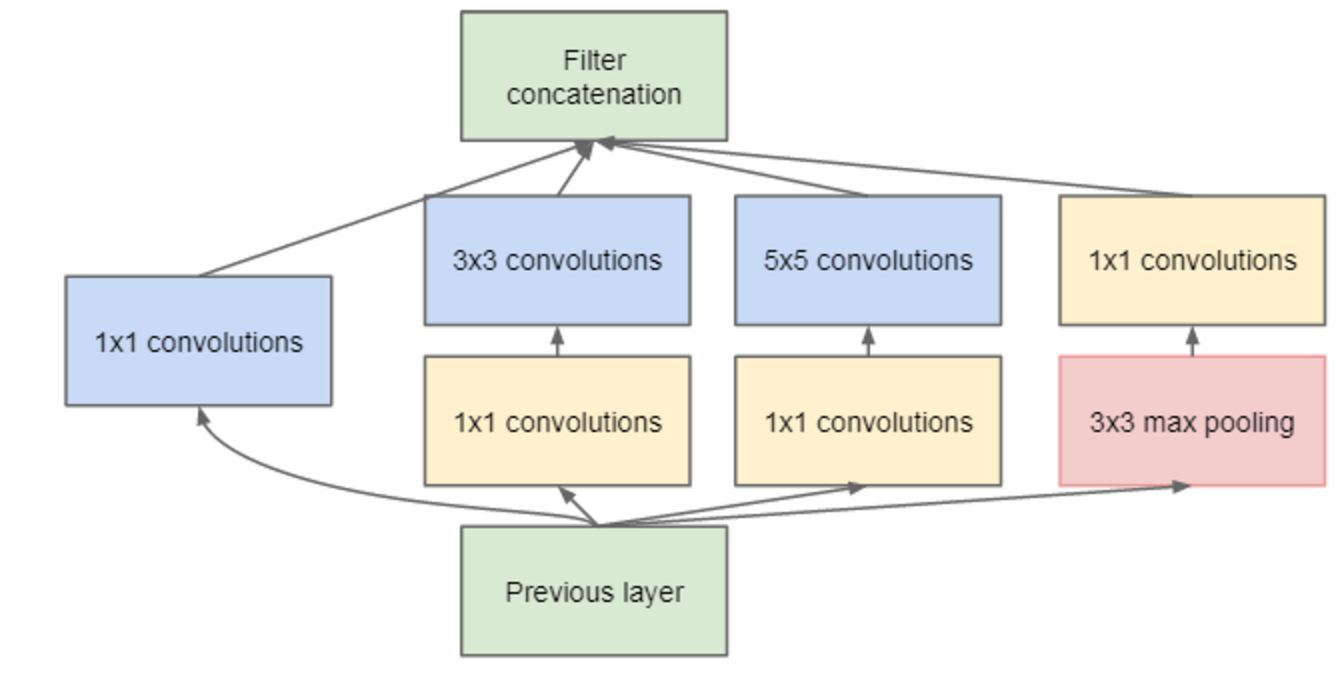
\includegraphics[width=0.8\textwidth]{Images/inception.png}
    \caption{Inception module \cite{googlenet}}
\end{figure}

And the complete GoogleNet architecture being:

\begin{figure}[H]
    \centering
    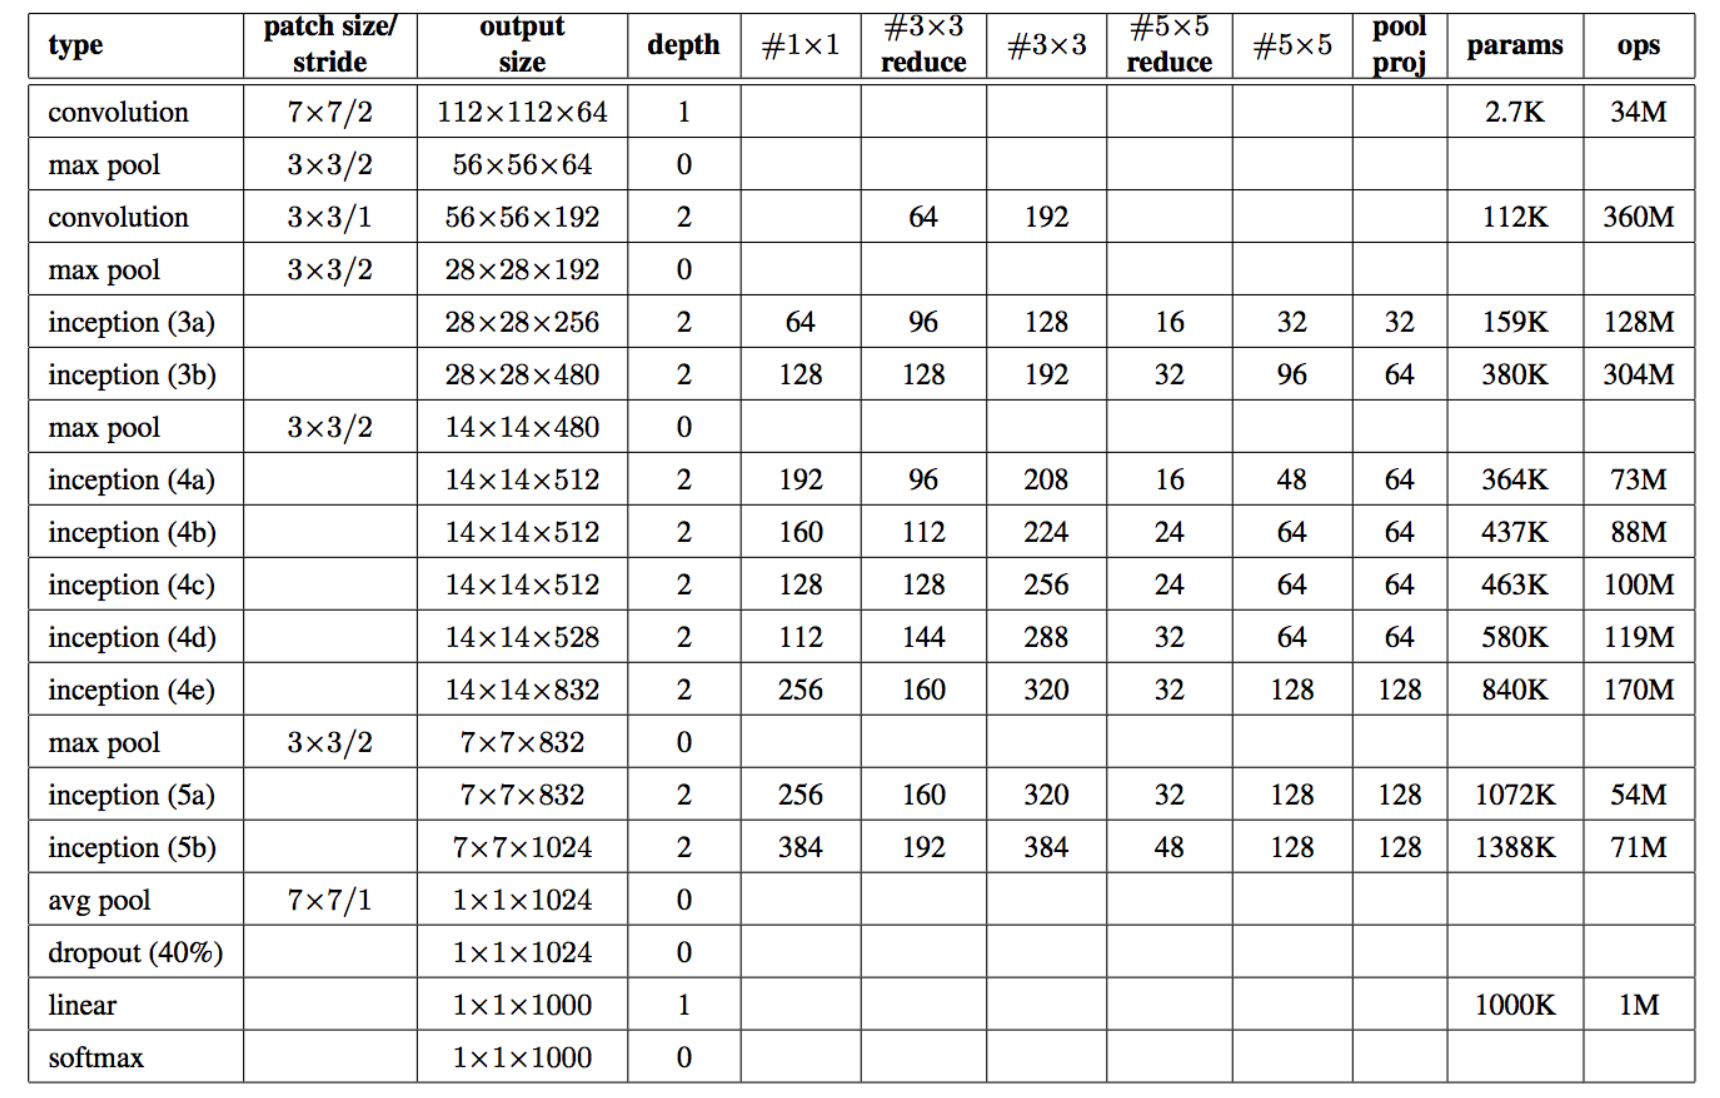
\includegraphics[width=\textwidth]{Images/googlenet.png}
    \caption{GoogleNet architecture\cite{googlenet}}
\end{figure}

The `\#$3\times3$ reduce' and `\#$5\times5$ reduce' refer to the dimensionality reduction with the $1\times1$ convolution. The `pool proj' refers to the depth of the $1\times1$ convolution following the $3\times3$ max-pool with stride 1 and zero-padding 1.

In our model, we got rid of the last linear layer and replaced it with another linear layer of size $(1, 1, 6)$ for the 6 different emotions.

\newpage
\subsection{Results}
Are the images enough to accurately determine the emotion conveyed by the user? We tried several machine learning models on the raw images, that were resized to a fixed size $(224, 224, 3)$. For now (need more time to train more data), the train set has 100 000 images and the test set has 20 000 images.
\begin{itemize}
    \item \textbf{Softmax regression}: with $\text{L}_2$ regularisation of $0.01$.
    \item \textbf{Random Forest Classification}: with $1000$ trees and max depth of $5$.
    \item \textbf{5-layer Convolutional Neural Network}: (each convolution is with stride 1, zero-padding to keep image size and followed by ReLU)
    \begin{itemize}[topsep=0pt]
        \itemsep-1em
        \item $3\times 3$ convolution, depth 8
        \item $3\times 3$ convolution, depth 16
        \item $2\times 2$ max-pooling with stride 2
        \item $3\times 3$ convolution, depth 32
        \item $2 \times 2$ max-pooling with stride 2
        \item Fully connected layer
        \item Fully connected layer
    \end{itemize}
    \item \textbf{Inception fine-tuned}: As described in 3.1.6, we retrained the final layer of the Inception model with:
    \begin{itemize}[topsep=0pt]
        \itemsep-1em
        \item 10 epochs
        \item Mini-batch size of 32
        \item Adam optimizer with learning rate $1\mathrm{e}{-5}$
    \end{itemize}
\end{itemize}

Here are the results, the measured accuracy being the fraction of correctly classified images on the test set:
\begin{table}[H]
\begin{center}
    \begin{tabular}{| l | l | p{5cm} |}
    \hline
    Model & Parameters & Test accuracy \\ \hline
    \textbf{Softmax regression} & $\text{L}_2$ reg: 0.01 & 0.40  \\ \hline
    \textbf{Random Forest} & 1000 trees & 0.50 \\ \hline
    \textbf{5-layer ConvNet} & architecture & 0.60 \\ \hline
    \textbf{Inception fine-tuned} & architecture & 0.65 \\
    \hline
    \end{tabular}
\end{center} 
\caption{Comparison of models using raw images}
\end{table}





